

\section{Sorting \XY}
\label{tree:open:xy}

\begin{figure}
	\centering
	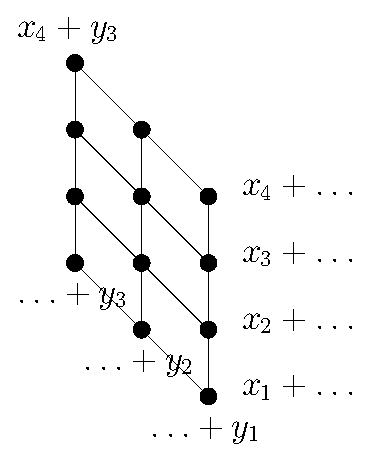
\includegraphics[height=0.2\textheight]{fig/open/x+y}
	\caption{Typical Hasse diagram for the Sorting \XY problem.}
	\label{fig:open:xy}
\end{figure}

Quoting \cite{orourke:2012:sortxy},

\begin{quotation}
Given two sets of numbers, each of size $n$, how quickly can the set of all
pairwise sums be sorted? In symbols, given two sets $X$ and $Y$, our goal is to
sort the set

$$ X + Y = \enum{x + y \st x \in X, y \in Y} $$

\end{quotation}

The earliest known reference is \citet*{fredman:1976}, who attributes
the problem to Elwyn Berlekamp. As we can see in \ref{fig:open:xy}, this
problem is a special case of \concept{SUPI}.

Several geometric problems are known to be ``Sorting-($X + Y$)-hard'' (see
\cite{barrera1996finding} and \cite{barequet2001polygon}). Specifically, there
is a subquadratic-time transformation from sorting $X + Y$ to each of the
following problems: computing the Minkowski sum of two orthogonal-convex
polygons, determining whether one monotone polygon can be translated to fit
inside another, determining whether one convex polygon can be rotated to fit
inside another, sorting the vertices of a line arrangement, or sorting the
interpoint distances between $n$ points in $\R^d$.

\citet{fredman:1976} also mentions an immediate application to multiplying sparse
polynomials. Let us explain. When we multiply
polynomials, each of the operands can be decomposed in terms. If polynomials
$p$ and $q$ are of size $n$ and $m$, then the resulting polynomial contains
$nm$ terms and the degree of each term in the resulting polynomial is the sum
of the degree of the operands terms. Since sparse polynomials are usually
stored in sorted order with respect to the degree of their terms, we can easily
see how the two problems are related.

While we have seen a lot of results on \concept{SUPI} the question of an
optimal $\BigO{n^2}$ algorithm still remains.

More references : \cite{orourke:2012:sortxy}, \cite{kahn:1995},
\cite{dietzfelbinger1989lower}, \cite{steiger1995pseudo},
\cite{lambert:1990}, \cite{erickson:1999},
\cite{bremner2012necklaces}.



